% Final storylines memo (5 November 2026): two routes out of the punishment dilemma,
% final Storyline 1 and Storyline 3, and the Discussion additions.
% Draft paragraphs are \input from paragraphs/, so the memo and the two final
% files always show the same text.
% Compile: pdflatex -> bibtex -> pdflatex x2 (from this directory).
\documentclass[11pt]{article}
\usepackage[T1]{fontenc}
\usepackage[a4paper,margin=2.2cm]{geometry}
\usepackage{times}
\usepackage{amsmath,amssymb,mathrsfs}
\usepackage[superscript,biblabel,nomove]{cite}
\usepackage{booktabs,tabularx,array,enumitem}
\usepackage[dvipsnames]{xcolor}
\usepackage[most]{tcolorbox}
\usepackage{tikz}
\usetikzlibrary{arrows.meta,positioning,fit,backgrounds}
\usepackage[hidelinks]{hyperref}
\newcommand{\JournalTitle}[1]{#1}
\setlength{\parskip}{0.45em}
\setlength{\parindent}{0pt}
\setlist{itemsep=0.15em,topsep=0.25em}
\definecolor{ink}{HTML}{23373B}
\definecolor{accent}{HTML}{A65A10}
\definecolor{orange}{HTML}{E07B16}
\definecolor{good}{HTML}{2F6E9E}
\definecolor{bad}{HTML}{C9506A}
\newtcolorbox{draft}[1]{colback=ink!3,colframe=ink!45,boxrule=0.4pt,arc=1.5pt,
  left=6pt,right=6pt,top=4pt,bottom=4pt,fonttitle=\small\bfseries,coltitle=ink,
  colbacktitle=ink!10,title={#1}}
\newtcolorbox{keypoint}{colback=accent!6,colframe=accent!70,boxrule=0.5pt,arc=1.5pt,
  left=6pt,right=6pt,top=4pt,bottom=4pt}
\newcolumntype{L}{>{\raggedright\arraybackslash}X}
\newcommand{\Rmap}{\mathscr{R}}
\title{\large\bfseries Final storylines for the Introduction\\[0.2em]
\normalsize Two routes out of the punishment dilemma, Storylines 1 and 3, and the Discussion additions}
\date{5 November 2026}
\begin{document}
\maketitle
\vspace{-1.5em}

\begin{keypoint}
\textbf{Summary.}
\begin{itemize}[leftmargin=1.2em]
\item \textbf{A framework for the field (Section~1).} Reputations are formed in two steps: an action is \emph{judged}, and the judgement \emph{revises} a reputation. The reputation an individual loses is the product of how often it is condemned (step~1) and how strongly each condemnation changes its reputation (step~2). This holds for wrongful condemnation of justified punishers, through disagreement or error, and for rightful condemnation of defectors. Existing remedies sort cleanly into the two steps. In our theory the product is explicit for rightful condemnation (Eq.~(3)), and the same slope $\Rmap'$ weighs wrongful condemnation. It yields four implications:
  \begin{itemize}[leftmargin=1.2em]
  \item the two routes are complementary;
  \item robust revision generates agreement;
  \item leniency at either step has a price;
  \item disputed evidence should be \emph{costly but not catastrophic}.
  \end{itemize}
\item \textbf{Storyline 1 (final).} Paragraph~1 introduces the two steps. Paragraph~2 ends with the two places where remedies can act. Paragraph~3 shows that the first step is well studied and that the second is treated symmetrically, which is the gap. 865 words.
\item \textbf{Storyline 3 (final, for \textit{Nature}).} The paper opens with everyday reputation and states the dilemma in plain language. The two steps become ``what observers know'' and ``how they revise what they believe''. The judgement problem is framed as a trade-off between two errors. 656 words, with no jargon before paragraph~4.
\item \textbf{Discussion additions.} One paragraph sets out the two routes, in a version for each storyline. A second carries the core of Storyline~2, agreement from private revision.
\end{itemize}
\end{keypoint}

% =============================================================================
\section{Two routes out of the punishment dilemma}

\subsection*{Two steps of reputation formation}
Every model of indirect reciprocity contains two steps, usually without naming them.
\begin{itemize}[leftmargin=1.2em]
\item \textbf{Step 1, judgement.} An observer judges an action against a norm. Under second-order norms, the judgement depends on the observer's view of the recipient.
\item \textbf{Step 2, revision.} The judgement updates the observer's view of the actor. In the standard model the update overwrites, and in ours it moves a record with inertia.
\end{itemize}
The punishment dilemma arises at step~1: a justified refusal is condemned by an observer who disagrees about the recipient. It propagates through step~2, because the condemnation overturns the punisher's standing. It then feeds back into step~1, because the punisher is now seen differently and disagreement spreads (Fig.~A).

\begin{center}
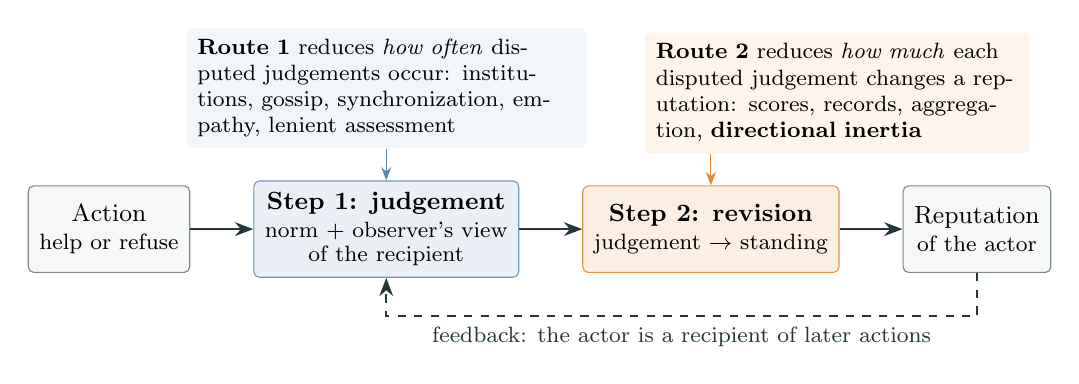
\begin{tikzpicture}[font=\small, node distance=8mm,
  box/.style={draw=ink!60, rounded corners=2pt, fill=ink!4, align=center, minimum height=11mm, inner sep=4pt},
  route/.style={rounded corners=2pt, align=left, font=\footnotesize, inner sep=4pt}]
\node[box] (act) {Action\\[-1pt]\footnotesize help or refuse};
\node[box, right=of act, fill=good!10, draw=good!70] (judge) {\textbf{Step 1: judgement}\\[-1pt]\footnotesize norm $+$ observer's view\\[-2pt]\footnotesize of the recipient};
\node[box, right=of judge, fill=orange!12, draw=orange!80] (rev) {\textbf{Step 2: revision}\\[-1pt]\footnotesize judgement $\to$ standing};
\node[box, right=of rev] (rep) {Reputation\\[-1pt]\footnotesize of the actor};
\draw[-{Stealth}, thick, ink] (act) -- (judge);
\draw[-{Stealth}, thick, ink] (judge) -- (rev);
\draw[-{Stealth}, thick, ink] (rev) -- (rep);
\draw[-{Stealth}, thick, ink, dashed] (rep.south) -- ++(0,-0.55) -| node[pos=0.25, below, font=\footnotesize] {feedback: the actor is a recipient of later actions} (judge.south);
\node[route, above=4mm of judge, text width=48mm, fill=good!6] (r1) {\textbf{Route 1} reduces \emph{how often} disputed judgements occur: institutions, gossip, synchronization, empathy, lenient assessment};
\node[route, above=4mm of rev, text width=46mm, xshift=16mm, fill=orange!8] (r2) {\textbf{Route 2} reduces \emph{how much} each disputed judgement changes a reputation: scores, records, aggregation, \textbf{directional inertia}};
\draw[-{Stealth}, good!80] (r1.south) -- (judge.north);
\draw[-{Stealth}, orange!90] ([xshift=-16mm]r2.south) -- (rev.north);
\end{tikzpicture}

\small\textbf{Fig.~A} | Two steps of reputation formation and the two routes out of the punishment dilemma.
\end{center}

\subsection*{Reputation loss is a product, for wrongful and rightful condemnation alike}
The reputation an individual loses depends on two factors: how often it is condemned (step~1) and how strongly each condemnation changes its reputation (step~2). The relation is general. It covers \emph{wrongful} condemnation of justified punishers, whether through disagreement about the recipient (the punishment dilemma) or through plain errors. It also covers \emph{rightful} condemnation of defectors. The punishment dilemma is the wrongful case, and deterrence is the rightful case.

In our theory, the relation is explicit for rightful condemnation. For a mutant that withholds help with small probability $\delta$, the reputation lost per unit of withheld cooperation is $\Delta\Phi^*\,\Rmap'(u_{\mathrm R}^*)$, and the invasion payoff has slope (Eq.~(3) of the manuscript)
\[
\Lambda'(0)=r_{\mathrm R}^*\Bigl[1-\frac{b}{c}\,\underbrace{\Delta\Phi^*}_{\text{step 1}}\;\underbrace{\Rmap'(u_{\mathrm R}^*)}_{\text{step 2}}\Bigr].
\]
\begin{itemize}[leftmargin=1.2em]
\item \textbf{Assessment contrast} $\Delta\Phi^*=\kappa\,[r+(p-q)(1-r)]$. A step-1 quantity: how differently cooperation and defection are judged, given the norm $(p,q)$, the errors and the observers' views $r$ of recipients.
\item \textbf{Slope} $\Rmap'$ of the reputation map. A step-2 quantity: how strongly a change in assessments moves a reputation.
\end{itemize}
The same slope weighs wrongful condemnations, since a small loss $\Delta u$ in positive assessments changes the reputation by about $\Rmap'(u)\,\Delta u$. This is the formal reason why route~2 shields defectors as well as punishers. The protection window has the same split (Eq.~(1)). The points $\Phi^*_{\mathrm D}$ and $\Phi^*_{\mathrm C}$ come from step~1, and whether $\Rmap$ lies above its chord between them is a property of step~2.

\textbf{Correction to the previous slide version.} An earlier slide stated the product as ``harm to justified punishers $\propto \Delta\Phi^*\times\Rmap'$''. That attribution was imprecise, because Eq.~(3) concerns deliberate withholding of help. The slides and the drafts now state the general relation, and the formula belongs to the Model section.

\subsection*{The literature sorted by step}
\begin{center}\small
\begin{tabularx}{\linewidth}{@{}>{\raggedright\arraybackslash}p{3.2cm} >{\raggedright\arraybackslash}p{4.2cm} L@{}}
\toprule
Step & Lever & Mechanisms \\
\midrule
1, judgement & Align information & Public institutions\cite{radzvilavicius2021}, gossip\cite{sommerfeld2007,kawakatsu2024}, opinion synchronization\cite{murase2024synchronization}, dual assessment\cite{tham2026} \\
 & Change perspective & Empathetic evaluation\cite{radzvilavicius2019} \\
 & Judge leniently & Generous assessment\cite{schmid2021}, the principle of generosity\cite{okada2020dilemmas}, norms prioritizing positive assessments\cite{okada2024} \\
\midrule
2, revision & Pool evidence symmetrically & Quantitative scores\cite{schmid2023}, simple records\cite{clark2020}, graded reputations\cite{tanabe2013,murase2022}, aggregation\cite{michelmata2024}, gradual dynamics\cite{yamamoto2025} \\
 & Directional inertia with graded expression & This work \\
\bottomrule
\end{tabularx}
\end{center}

\subsection*{Four implications}
Each implication is labelled with the support it has.
\begin{enumerate}[leftmargin=1.5em]
\item \textbf{The routes are complementary} (conceptual, consistent with known results). A shortfall at one step can be offset at the other. Under public information, step-1 agreement makes fragile revision harmless, which is the classical leading-eight result. Under private information, robust revision can compensate for disagreement, which is our result.
\item \textbf{Robust revision generates agreement} (supported by Fig.~2). Revision acts at step~2, yet it reduces disagreement at step~1 through the feedback loop. Reliable private verdicts coincide, because two independent observers disagree with probability $2r(1-r)$. The condition is that inertia is placed in the direction that separates the assessments of cooperators from those of defectors. If it is not, agreement forms on the wrong verdict (one-step Shunning).
\item \textbf{Leniency has a price at either step} (supported by Fig.~5a; for generosity, see Schmid et al.\cite{schmid2021}). Anything that lowers the reputational impact of negative evidence, whether lenient judgement or tolerant revision, also lowers the cost of deliberate defection. In the formula above, a small $\Delta\Phi^*$ or a small $\Rmap'$ both make $\Lambda'(0)>0$ more likely. Inertia separates wrongful from rightful condemnation only by pattern. It absorbs isolated condemnations, which are typical of errors, but not repeated ones. Occasional defection produces isolated condemnations, which is why it slips through.
\item \textbf{Costly but not catastrophic} (design principle, supported by Fig.~5). The impact of a single negative assessment has two parts.
  \begin{itemize}[leftmargin=1.2em]
  \item Whether it can overturn a reputation. This is the global shape of $\Rmap$, controlled by the depths. Suppressing it stops cascades.
  \item What it costs at the margin. This is the slope $\Rmap'(1)=1-\alpha$, controlled by the strength. Keeping it positive keeps deterrence.
  \end{itemize}
  Standard updating makes every disputed judgement catastrophic. Symmetric tolerant rules make it nearly costless. Inertia with partial consequences is costly but not catastrophic. The right direction mirrors the errors that step~1 produces under each norm. Norms and revision rules should therefore be designed together.
\end{enumerate}

\subsection*{Why this advances the field}
\begin{itemize}[leftmargin=1.2em]
\item It turns a list of disparate remedies into two factors, so that mechanisms can be compared by which factor they reduce and at what price.
\item It explains why agreement-based and robustness-based remedies can substitute for each other, and why robust revision can produce agreement without communication.
\item It identifies a trade-off shared by every lenient remedy and a design rule that escapes it.
\item It yields testable predictions for experiments that measure the two factors separately:
  \begin{itemize}[leftmargin=1.2em]
  \item how often people dispute a justified refusal;
  \item how strongly one disputed act changes their impression of the punisher, and whether a single lapse is treated as costly but not catastrophic.
  \end{itemize}
\end{itemize}

\textbf{Where it appears.}
\begin{itemize}[leftmargin=1.2em]
\item \textbf{Storyline~1:} paragraphs~1--3 (the two steps) and the Discussion paragraph on the two routes.
\item \textbf{Storyline~3:} paragraph~2 (``what observers know'' and ``how they revise what they believe''), paragraph~3, and the Discussion paragraph.
\item \textbf{Figure:} Fig.~A could become a schematic panel of Fig.~1 or an Extended Data figure.
\end{itemize}

% =============================================================================
\section{Storyline 1, final}

\textbf{Tailoring.}
\begin{itemize}[leftmargin=1.2em]
\item Paragraph~1 now names the two steps (``Observers judge each action against a social norm, and they revise their view of the actor in light of that judgement'').
\item Paragraph~2 ends with the product (``how often \dots\ and how strongly \dots'') and the two places where remedies act.
\item Paragraph~3 sorts the literature into the two steps, so the gap appears where the second step is treated symmetrically.
\item Paragraph~5 notes that inertia, acting at the second step, also reduces disagreement.
\end{itemize}
The paragraphs are 153, 181, 197, 147 and 187 words long.

\begin{draft}{Storyline 1, paragraph 1}% Storyline 1 (final), paragraph 1: classical result, the two steps of reputation formation, the central problem.
Cooperation among unrelated individuals is sustained in part by reputation\cite{milinski2016,nowak2005}. By helping others, individuals improve their standing and become more likely to receive help from third parties, a mechanism known as indirect reciprocity\cite{nowak1998,leimar2001,wedekind2000,milinski2002}. Reputations are built in two steps. Observers judge each action against a social norm, and they revise their view of the actor in light of that judgement\cite{ohtsuki2004,santos2018}. Theory has identified norms that make reputation-based cooperation evolutionarily stable\cite{panchanathan2003,ohtsuki2004}, most notably the leading-eight norms, which sustain cooperation when reputations are public, even in the presence of occasional errors\cite{ohtsuki2004,ohtsuki2006}. These results rest on agreement about who is good and who is bad. When reputations are private and assessments are noisy, individuals hold different views of the same person\cite{takahashi2006,uchida2010}, and most leading-eight norms no longer maintain stable cooperation\cite{hilbe2018,okada2018,perret2021,fujimoto2023}. Reputations must then remain both accurate and shared, distinguishing those who cooperate from those who do not while different observers largely agree about who is who\cite{fujimoto2022,murase2024synchronization}.
\end{draft}
\begin{draft}{Storyline 1, paragraph 2}% Storyline 1 (final), paragraph 2: the punishment dilemma and the two steps at which remedies can act.
The difficulty is sharpest for the norms that sustain cooperation under public information. Under these norms, a discriminator who refuses to help an individual in bad standing keeps its own good standing, because the refusal counts as justified punishment\cite{panchanathan2003,ohtsuki2004,okada2020dilemmas}. This exemption works only if the observer shares the donor's view of the recipient, which under private assessment is often not the case. An observer who still regards the recipient as good sees an unjustified refusal and condemns the discriminator. Disagreement about one individual thereby becomes disagreement about those who act towards it, and it spreads through the population\cite{hilbe2018,uchida2013,radzvilavicius2019}. Discriminators thus face a punishment dilemma. Withholding help from defectors protects cooperation against exploitation, yet each act of punishment risks their own reputation in the eyes of observers who disagree\cite{okada2020dilemmas,michelmata2024,pires2025}. The harm done by such disputed judgements depends on how often they occur and on how strongly each one changes a reputation. Remedies can therefore act at either step of reputation formation, on how actions are judged or on how judgements are turned into reputations, provided that genuine defectors still lose their standing.
\end{draft}
\begin{draft}{Storyline 1, paragraph 3}% Storyline 1 (final), paragraph 3: the first step is well studied; the second step and the gap.
Most remedies act on the first step. Public institutions, gossip, empathetic evaluation and the synchronization of private opinions reduce how often observers disagree\cite{radzvilavicius2021,kawakatsu2024,radzvilavicius2019,murase2024synchronization,tham2026}, and generous or lenient assessment reduces how often a disputed act is condemned\cite{schmid2021,okada2024}. At the second step, the standard framework lets each new assessment replace an individual's image, so a single disputed act of punishment overturns a standing built over many interactions\cite{ohtsuki2004,hilbe2018}. Quantitative scores, simple records, graded reputations and the aggregation of several observations soften this impact and can make cooperation more robust\cite{schmid2023,clark2020,tanabe2013,murase2022,michelmata2024,yamamoto2025}. Most of them, however, treat reputational change as a single symmetric process, in which positive and negative evidence enter through the same score, threshold or observation window and affect treatment only once a threshold is crossed. Human evaluation departs from both features. Impressions of others are revised asymmetrically, although the direction of the asymmetry depends on context\cite{skowronski1989,slovic1993,mendesiedlecki2013diagnostic,siegel2018}. Institutions, too, grade their response and treat the two directions differently, escalating sanctions only with repeated violations\cite{ostrom1990,cox2010} and restoring an offender's standing only after years without a further offence\cite{blumstein2009}. How the direction of reputational change and the treatment of incomplete evidence affect the punishment dilemma, and with it the evolution of cooperation, remains unclear.
\end{draft}
\begin{draft}{Storyline 1, paragraph 4}% Storyline 1 (final), paragraph 4: approach.
Here, we develop a model of indirect reciprocity in which reputations have inertia, and in which this inertia can differ between losing and regaining standing (Fig.~1). An established reputation changes only after a run of contrary assessments. Negative assessments move an individual in good standing through a sequence of warning states before the reputation turns bad, and positive assessments move an individual in bad standing through recovery states before it turns good. The two paths can differ in length, so that losing and regaining standing may require different amounts of evidence. Each intermediate state is interpreted as good or bad with a probability that sets how strongly incomplete evidence already affects treatment. The model thus treats two properties of reputational change as separate design choices, namely how much evidence is needed to change a reputation in each direction and how incomplete evidence is expressed in the meantime.
\end{draft}
\begin{draft}{Storyline 1, paragraph 5}% Storyline 1 (final), paragraph 5: findings and implication.
We find that the allocation of inertia between the two directions, rather than its total amount, determines whether private observers agree with one another and still distinguish cooperators from defectors. Although inertia acts only on how judgements are turned into reputations, it also reduces disagreement among observers, who share no information. The beneficial direction depends on the norm. Compact architectures, selected solely by these reputational criteria, make cooperation stable and easy to reach under each of four classical norms (Scoring, Shunning, Stern Judging and Simple Standing). At the same depth, inertia placed on the wrong path can leave no cooperation at all. We further show that the tolerance that protects justified punishers can also shelter opportunists who defect only occasionally, a vulnerability that the aggregation and score-based rules we test share. Allowing warning states to carry partial consequences closes this loophole for the opportunistic strategies we consider, while cooperation remains high. Reputation-based cooperation therefore depends not only on which behaviours a society judges as good, but also on how readily it revises those judgements in each direction and on how it treats individuals before a judgement changes.
\end{draft}

% =============================================================================
\section{Storyline 3, final (for a multidisciplinary journal)}

\textbf{Tailoring for \textit{Nature}.}
\begin{itemize}[leftmargin=1.2em]
\item Paragraph~1 opens with everyday reputation (``From village communities to online marketplaces'') and avoids technical terms.
\item Paragraph~2 states the dilemma in plain words and ends with the product split into ``what observers know'' and ``how they revise what they believe''.
\item Paragraph~3 turns the second factor into a general problem of judgement with a trade-off between two errors.
\item Paragraph~4 opens with ``Here, we show'' and uses intuitive labels (``under suspicion or on probation'') for the intermediate states.
\item Paragraph~5 ends with the one-sentence message.
\item Total 656 words. Norm names and model terms appear only from paragraph~4 onward.
\end{itemize}

\begin{draft}{Storyline 3, paragraph 1}% Storyline 3 (final, for a multidisciplinary journal), paragraph 1: broad opening.
From village communities to online marketplaces, people decide whom to help on the basis of what they know about others' past conduct\cite{milinski2016,tadelis2016}. Those who help gain a good reputation, and a good reputation attracts help from third parties. This feedback, known as indirect reciprocity, can sustain cooperation among strangers who may never meet again\cite{nowak1998,nowak2005,wedekind2000,milinski2002}. Theory has identified social norms under which it is evolutionarily stable\cite{leimar2001,panchanathan2003,ohtsuki2004,ohtsuki2006}, but these results assume that everyone agrees about who is good. In reality, each person forms a private view from noisy and incomplete observations\cite{takahashi2006,uchida2010}, and once views diverge, most of these norms no longer sustain cooperation\cite{hilbe2018,okada2018,perret2021,fujimoto2023}.
\end{draft}
\begin{draft}{Storyline 3, paragraph 2}% Storyline 3 (final), paragraph 2: the punishment dilemma in plain terms; knowledge versus revision.
The trouble lies in punishment. Stable norms allow people to refuse help to those in bad standing without losing their own good standing, because the refusal is seen as justified\cite{panchanathan2003,ohtsuki2004,okada2020dilemmas}. Whether a refusal looks justified, however, depends on the observer's own view of the person refused. An observer who still regards that person as good condemns the punisher, and disagreement about one individual spreads to those who act towards it\cite{hilbe2018,uchida2013,radzvilavicius2019}. Those who punish defectors thus put their own reputation at risk, a punishment dilemma that undermines the sanctions on which cooperation depends\cite{okada2020dilemmas,michelmata2024,pires2025}. The harm has two components, how often justified punishers are condemned and how much each condemnation changes their reputation. The first depends mainly on what observers know, the second on how they revise what they believe.
\end{draft}
\begin{draft}{Storyline 3, paragraph 3}% Storyline 3 (final), paragraph 3: information remedies, the remaining problem of judgement, the gap.
Most proposed remedies act on what observers know. Public institutions, gossip and the synchronization of opinions bring observers to a common view\cite{radzvilavicius2021,kawakatsu2024,murase2024synchronization,tham2026}, and the aggregation of several observations gives each observer more evidence to judge from\cite{michelmata2024}. Better information reduces disputed judgements, but it cannot remove the errors that make every judgement fallible\cite{hilbe2018,murase2023}. What remains is a problem of judgement, namely how a standing verdict about another person should be revised as new evidence arrives. Any revision rule must balance two errors, condemning cooperators on disputed evidence and excusing defectors whose misconduct is not yet conclusive. Human institutions often strike this balance through procedure. They escalate sanctions only with repeated violations\cite{ostrom1990,cox2010} and restore an offender's standing only after a period of good conduct\cite{blumstein2009}, and people likewise revise their impressions of others asymmetrically\cite{skowronski1989,slovic1993,mendesiedlecki2013diagnostic,siegel2018}. Models of indirect reciprocity, by contrast, mostly revise reputations through a single symmetric rule, whether the latest assessment, a score or a fixed window of observations\cite{ohtsuki2004,hilbe2018,schmid2023,michelmata2024}. How such revision rules shape the punishment dilemma, and how they should be designed, remains open.
\end{draft}
\begin{draft}{Storyline 3, paragraph 4}% Storyline 3 (final), paragraph 4: approach.
Here, we show that the way private judgements are revised can sustain cooperation despite the punishment dilemma, without any shared information. We develop a model of indirect reciprocity in which judgements have inertia (Fig.~1). An established reputation changes only after a run of contrary assessments, and the run required to lose standing can differ from the run required to regain it. While evidence accumulates, an individual under suspicion or on probation can already face partial consequences, depending on how strongly these intermediate states are expressed. Observers share no information and update on one observation at a time, so any agreement among them must emerge from how they revise their judgements.
\end{draft}
\begin{draft}{Storyline 3, paragraph 5}% Storyline 3 (final), paragraph 5: findings and broad implication.
We find that the direction of revision, rather than the amount of evidence it requires, decides whether private observers agree with one another and still tell cooperators from defectors. The beneficial direction mirrors the kind of misjudgement that private assessment produces under each norm, and rules selected solely by these reputational criteria make cooperation stable and easy to reach under four classical norms. The same amount of inertia placed in the wrong direction can eliminate cooperation altogether. Rules that protect cooperators from disputed evidence, however, can also shelter opportunists who defect only occasionally, a weakness shared by the aggregation and score-based rules we test. Letting suspicion carry partial consequences restores deterrence while cooperation remains high. Sustaining cooperation through private reputations is therefore not only a matter of what individuals know about each other, but also of how they revise what they believe.
\end{draft}

% =============================================================================
\section{Discussion additions}

The first paragraph replaces, or merges with, the current Discussion paragraph on the vulnerability to opportunism, which makes a related point more narrowly. The second carries Storyline~2 and can follow the current paragraph on agreement and accuracy.

\begin{draft}{Two routes, Storyline 1 version}% Discussion paragraph for Storyline 1: the two routes out of the punishment dilemma.
% In the manuscript, replace Eq.~(3) by Eq.~\eqref{eq:lambda-slope} and Fig.~5a by Fig.~\ref{fig:opportunism}a.
Our analysis suggests a general way to organize remedies for the punishment dilemma. The harm that disputed judgements do to justified punishers depends on how often such judgements occur and on how strongly each one changes a reputation. Institutions, gossip, synchronization and generous assessment act on the first factor\cite{radzvilavicius2021,kawakatsu2024,murase2024synchronization,schmid2021}, whereas scores, aggregation and inertia act on the second\cite{schmid2023,michelmata2024}. The same separation appears in our theory. Near a resident population, the reputational cost of withholding help is the product of a term from the first step, the assessment contrast, which measures how differently observers judge cooperation and defection, and a term from the second step, the slope of the reputation map, which measures how strongly a change in assessments moves a reputation (Eq.~(3)). The two routes are therefore complementary. Weak agreement can be offset by robust revision, as in our model, and fragile revision does little harm when information is public. Leniency, however, has a price at either step. Generous assessment and tolerant revision both protect deliberate defectors as well as justified punishers\cite{schmid2021}, as our comparison of inertia, aggregation and scores shows (Fig.~5a). A reputation system should therefore separate whether a single negative assessment can overturn a reputation, which inertia suppresses, from what it costs at the margin, which partial consequences restore. Disputed evidence should be costly but not catastrophic.
\end{draft}
\begin{draft}{Two routes, Storyline 3 version}% Discussion paragraph for Storyline 3: knowledge versus revision as two routes out of the dilemma.
% In the manuscript, replace Eq.~(3) by Eq.~\eqref{eq:lambda-slope} and Fig.~5a by Fig.~\ref{fig:opportunism}a.
The distinction between what observers know and how they revise what they believe offers a general way to organize remedies for the punishment dilemma. The harm that disputed judgements do to justified punishers depends on how often such judgements occur and on how strongly each one changes a reputation. Institutions, gossip, synchronization and generous assessment act on the first factor\cite{radzvilavicius2021,kawakatsu2024,murase2024synchronization,schmid2021}, whereas scores, aggregation and inertia act on the second\cite{schmid2023,michelmata2024}. The same separation appears in our theory. Near a resident population, the reputational cost of withholding help is the product of the assessment contrast, which measures how differently observers judge cooperation and defection, and the slope of the reputation map, which measures how strongly a change in assessments moves a reputation (Eq.~(3)). The two routes are therefore complementary. Weak agreement can be offset by robust revision, as in our model, and fragile revision does little harm when information is public. Leniency, however, has a price on either route. Generous assessment and tolerant revision both protect deliberate defectors as well as justified punishers\cite{schmid2021}, as our comparison of inertia, aggregation and scores shows (Fig.~5a). A revision rule should therefore separate whether a single negative assessment can overturn a reputation, which inertia suppresses, from what it costs at the margin, which partial consequences restore. Disputed evidence should be costly but not catastrophic.
\end{draft}
\begin{draft}{Agreement from private revision, core of Storyline 2, either storyline (180 words)}% Discussion paragraph carrying the core of Storyline 2 (agreement from private revision), for either storyline.
% In the manuscript, refer to Fig.~\ref{fig:recognition} for the Shunning example.
Our results also bear on how agreement about reputations arises. Agreement is usually attributed to mechanisms that align information across observers, such as institutions, gossip and opinion synchronization\cite{radzvilavicius2021,kawakatsu2024,murase2024synchronization}, or to observers who draw on several observations at once\cite{michelmata2024}. In our model, observers share nothing and update on one observation at a time, yet they largely agree. Two independent observers who each regard an individual as good with probability $r$ disagree with probability $2r(1-r)$, so agreement follows whenever private judgements become reliable. Under the punishment dilemma, reliability is not automatic, because the assessments an individual receives depend on what observers think of its recipients. Inertia produces it when it is placed in the direction that separates the assessments of cooperators from those of defectors. Otherwise observers can agree on the wrong verdict, as under one-step Shunning, where they regard nearly everyone as bad (Fig.~2). Agreement through private revision complements information sharing rather than replacing it. It remains available where shared information is costly or untrusted, as in polarized societies\cite{iyengar2019,michelmata2024}, and it can be combined with institutions or gossip where they exist.
\end{draft}

% =============================================================================
\section{The choice between Storylines 1 and 3}

\begin{center}\small
\begin{tabularx}{\linewidth}{@{}>{\raggedright\arraybackslash}p{2.8cm} L L@{}}
\toprule
& \textbf{Storyline 1} & \textbf{Storyline 3} \\
\midrule
One-line message & How a society revises its judgements in each direction matters as much as which behaviours it judges good & Cooperation depends not only on what individuals know about each other, but also on how they revise what they believe \\
Frame & Two steps of reputation formation; the second is treated symmetrically & Information versus judgement; judgement is a trade-off between two errors \\
Audience & Indirect reciprocity and evolutionary game theory & Broad (social science, institutions, online and multi-agent systems) \\
Science & \multicolumn{2}{l}{Identical: same model, same results, same Discussion additions} \\
Venue & \textit{PNAS}, \textit{Nat.\ Commun.} & \textit{Nature}, \textit{Nat.\ Hum.\ Behav.} \\
Risk & Reads as a model extension & Broad claims must be carried by the Discussion \\
\bottomrule
\end{tabularx}
\end{center}

\textbf{To check before finalizing.}
\begin{itemize}[leftmargin=1.2em]
\item Yamamoto et al.\ 2025\cite{yamamoto2025}: whether it lets gains and losses differ or grades treatment. I could not access it from here.
\item The Discussion's ``mirrors the errors'' argument supports one sentence in Storyline~3, paragraph~5. Keep both consistent.
\item That Schmid et al.\ 2021\cite{schmid2021} and Okada et al.\ 2024\cite{okada2024} are best described as lenient \emph{assessment}. This is how they are placed in the table and in Storyline~1, paragraph~3.
\end{itemize}

\bibliographystyle{../../latex_file/naturemag-doi}
\bibliography{../../latex_file/references}
\end{document}
